% !TEX root = ../presentation.tex
% !BIB program = biber
% !TEX program = xelatex

\section{Introduction}

\begin{frame}
    \frametitle{Healthcare}
    \begin{quotation}
        \noindent\centering
        Healthcare is the improvement of health via the \highlight{prevention}, \highlight{diagnosis}, \highlight{treatment}, \highlight{amelioration} or \highlight{cure} of {\color{theme-green}disease}, {\color{theme-green}illness}, {\color{theme-green}injury}, and {\color{theme-green}other physical and mental impairments} in people.
    \end{quotation}
\end{frame}


% \begin{frame}
%     \frametitle{Medical dialogue}
%     \begin{figure}
%         \centering
%         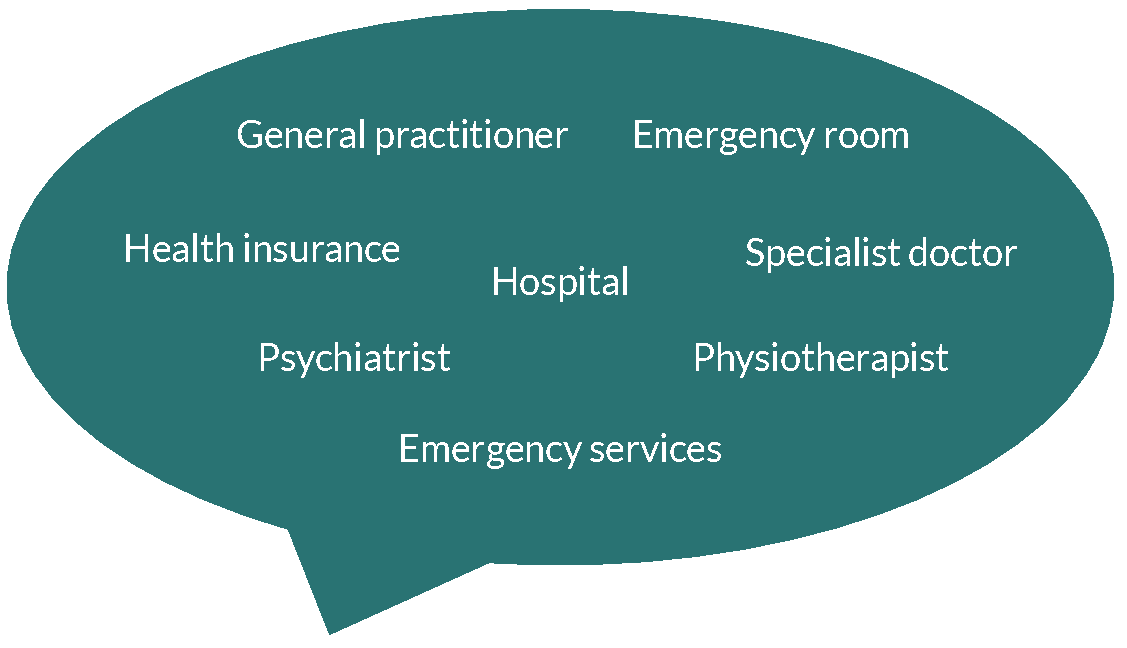
\includegraphics[width=0.7\paperwidth]{figures/speech_bubble.pdf}
%     \end{figure}

%     \note[item]{Healthcare sector is a complex system}
% \end{frame}
% \begin{frame}
%     \frametitle{Medical dialogue}
%     \begin{figure}
%         \centering
%         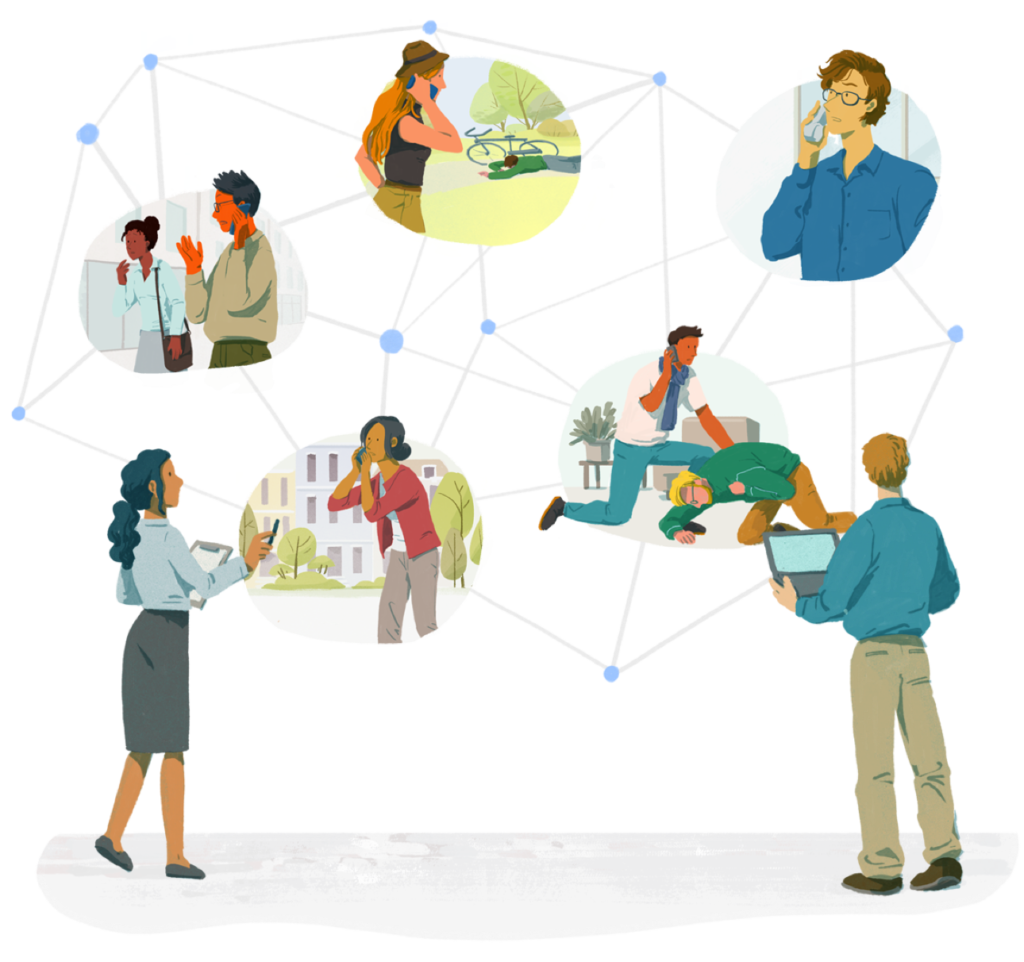
\includegraphics[width=0.95\textheight]{figures/corti_sketch_conversations.png}
%     \end{figure}
% \end{frame}


\begin{frame}[t]
    \frametitle{Medical dialogue}
    \begin{columns}[t]
        \begin{column}{0.4\textwidth}
            \begin{itemize}
                \item <2> General practitioner
                \item <2> Nurse
                \item <2> Midwife
                \item <2> Emergency medical dispatcher
                \item <2> Paramedic
                \item <2> Emergency room
                \item <2> Health insurance
            \end{itemize}
        \end{column}
        \begin{column}{0.6\textwidth}
            \vspace{-2em}
            \begin{figure}[t]
                \centering
                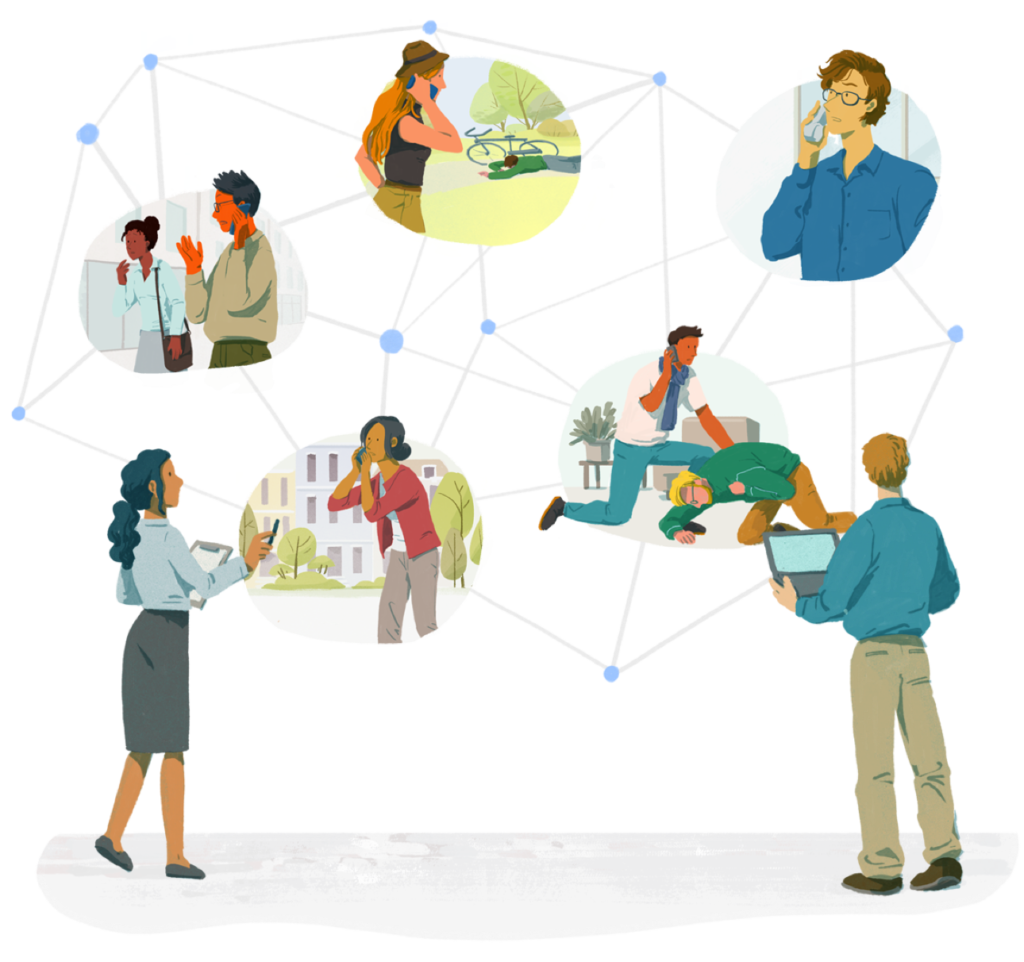
\includegraphics[width=0.9\textwidth]{figures/corti_sketch_conversations.png}
            \end{figure}
        \end{column}
    \end{columns}
\end{frame}


\begin{frame}
    \frametitle{Errors in medical dialogue}
    \begin{columns}
        \begin{column}{0.5\textwidth}
            \begin{itemize}
                \item <1-> Communication is everywhere in healthcare. 
                \item <1-> It is complex, involving multiple participants, different contexts, and different purposes.
                \vspace{1em}
                \item <2-> \highlight{Adverse events}: Failure of communication is a leading cause of medical error contributing to two out of three adverse events \cite{starmer_changes_2014}.
                \item <2-> \highlight{Preventability}: A considerable fraction of all hospital admissions have preventable adverse outcomes\footnote<2>{9\% to 16.6\% in AU, NZ, UK, DK.} \cite{carver_medical_2024}.
            \end{itemize}
        \end{column}
        \begin{column}{0.5\textwidth}
            \begin{figure}
                \centering
                
\includegraphics[width=0.95\textwidth]{figures/corti_sketch_emergency.png}
            \end{figure}
        \end{column}
    \end{columns}
\end{frame}


\begin{frame}
    \frametitle{Documenting medical encounters}
    \begin{columns}
        \begin{column}{0.5\textwidth}
            \begin{itemize}
                \item <1,2> Documentation is a central part of healthcare.
                \item <1,2> E.g. patient records, insurance claims, billing, research, training, legal purposes.
                \vspace{1em}
                \item <2> \highlight{Time-consuming}: Physicians spend 34-37\% of their time on documentation \cite{joukes_time_2018, tipping_where_2010, sinsky_allocation_2016}\footnote<2>{Ambulatory care across four specialties in four states and tertiary care at an academic medical center.}.
                \item <2> \highlight{Varying quality}: Discharge summaries almost never meet \emph{all} timeline, transmission, and content criteria. \cite{horwitz_comprehensive_2013}\footnote<2>{Outpatient visits, Yale-New Haven Hospital.}
            \end{itemize}
        \end{column}
        \begin{column}{0.5\textwidth}
            \begin{figure}
                \centering
                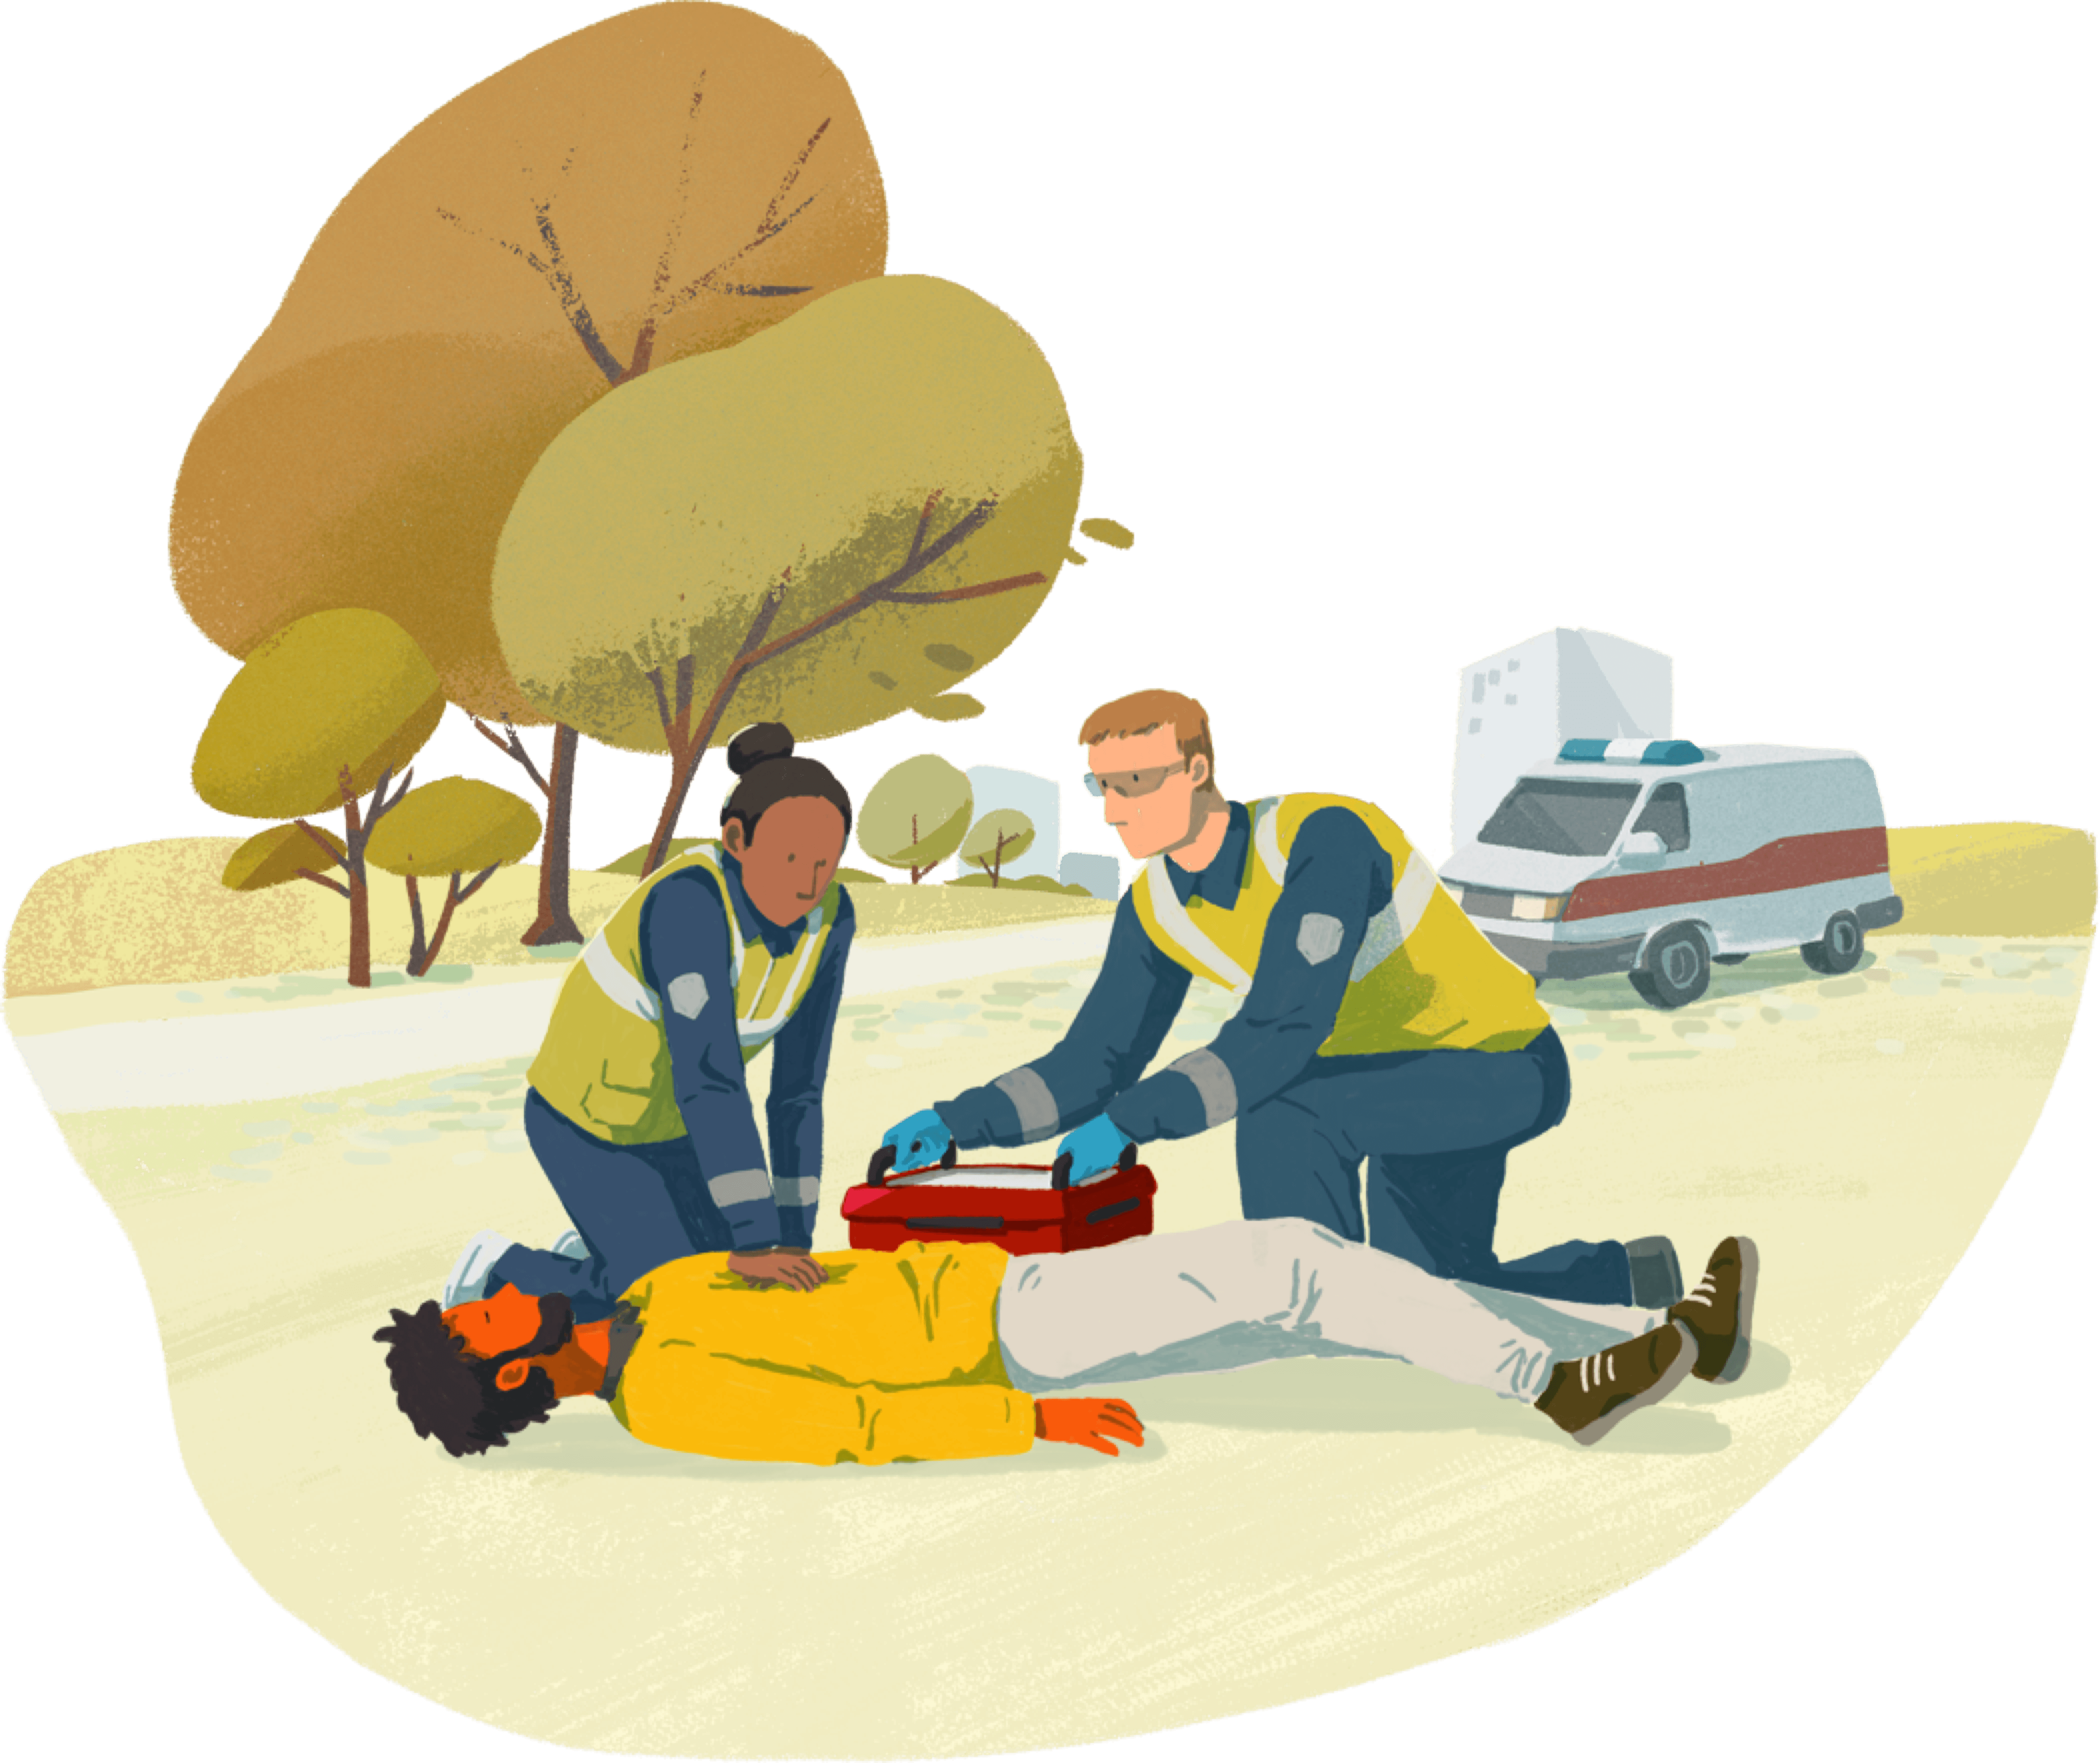
\includegraphics[width=0.95\textwidth]{figures/corti_sketch_responders.png}
            \end{figure}
        \end{column}
    \end{columns}
    \note[item]{Documentation is essential for a number of purposes but is very time-consuming and imperfect}
\end{frame}
    

\begin{frame}
    \frametitle{How might machine learning help?}
    \begin{columns}
        \begin{column}{0.35\textwidth}
            \begin{itemize}
                \item <1-> \highlight{Assist} with documentation.
                \item <1-> \highlight{Augment} communication.
                \item <1-> \highlight{Improve} decision-making.
                \vspace{1em}
                \item <2-> \highlight{Reduce} the impact of medical errors and adverse events.
                \item <2-> \highlight{Free up} time spent on documentation for patient care.
            \end{itemize}
        \end{column}
        \begin{column}{0.65\textwidth}
            \centering
            \includegraphics[width=0.95\textwidth]{figures/corti_sketch_office.png}
        \end{column}
    \end{columns}
\end{frame}


\begin{frame}
    \frametitle{Reliability of machine learning systems}
    \begin{itemize}
        \item <1-> \highlight{Data}: Quality, quantity, diversity, bias, privacy, ethics.
        \item <2-> \highlight{Task}: Context, domain, language, culture, purpose.
        \vspace{1em}
        \item <3-> \highlight{Interpretability} of how a model works (transparency, accountability, regulation).
        \item <4-> \highlight{Explainability} of model predictions (trust, understanding, feedback).
        \item <5-> \highlight{Fairness} in treatment of different groups of people.
        \item <6-> \highlight{Robustness} to noise, outliers, distribution shift, and adversarial attacks.
    \end{itemize}
\end{frame}


\tikzstyle{mybox} = [fill, rounded corners, minimum width=140, minimum height=20]
\tikzstyle{myrect} = [fill]

\begin{frame}
    \frametitle{Building a decision-support system}
    \begin{columns}
        \begin{column}{0.6\textwidth}
            Modular approach:
            \begin{itemize}
                \item \highlight{Input}: Speech or text (potentially video, tabular data, images, etc.).
                \item \highlight{Parsing the input}: Representation learning and speech recognition.
                \item \highlight{Output}: Predictions (suggesting, summarizing, classifying, etc.).
            \end{itemize}
        \end{column}
        \begin{column}{0.4\textwidth}
            \resizebox{!}{0.8\textheight}{%
            \begin{tikzpicture}[x=1cm,y=1cm]
                \node<6> [mybox, fill=presentation_orange] at (0,5) (predictions) {};
                \foreach \i in {-11,...,11} {
                    \fill<6>[myrect, fill=presentation_orange_shaded] (0.2*\i,4.8) rectangle ++(0.1,0.4);
                }
                \node<6> [] at (0,5) {\small\textsc{predictions}};
    
                \node<5> [mybox, fill=black!10] at (0,4) (downstream) {\small\textsc{downstream model}};
    
                \node<4> [mybox, fill=presentation_blue] at (0,3) (text) {};
                \foreach \i in {-11,...,11} {
                    \fill<4>[myrect, fill=presentation_blue_shaded] (0.2*\i,2.8) rectangle ++(0.1,0.4);
                }
                \node<4> [] at (0,3) {\small\textsc{text}};
    
                \node<3> [mybox, fill=black!10] at (0,2) (recognition) {\small\textsc{speech recognition}};
    
                \node<2> [mybox, fill=black!10] at (0,1) (representation) {\small\textsc{representation learning}};
    
                \node<1> [mybox, fill=presentation_green] at (0,0) (speech) {};
                \foreach \i in {-11,...,11} {
                    \fill<1>[myrect, fill=presentation_green_shaded] (0.2*\i,-0.2) rectangle ++(0.1,0.4);
                }
                \node<1> [] at (0,0) {\small\textsc{speech}};
    
                \node<7> [draw, rectangle, rounded corners, line width=0.15cm, presentation_red, fit=(speech)(representation)(recognition)(text)(predictions), inner sep=10pt] (uncertainty) {};
                \node<7> [above] at (uncertainty.north) {\small\textsc{uncertainty}};
            \end{tikzpicture}
        }
        \end{column}
    \end{columns}
\end{frame}
